% Source: graduate-coursework/Sp26/CSCE763/Course_Assignments/Project/project_proposal.tex
% Description: Otsu thresholding with region property analysis. Seed-point detection handles the small-target problem before shape-based filtering.

\documentclass[border=4pt]{standalone}
\usepackage{amsmath}
\usepackage{amssymb}
\usepackage{graphicx}
\usepackage{tikz}
\usepackage{xcolor}
\usetikzlibrary{positioning, arrows.meta, calc, fit, backgrounds, decorations.pathreplacing}

\definecolor{USC_Garnet}{HTML}{73000A}
\definecolor{USC_Black10}{HTML}{ECECEC}
\definecolor{USC_Black70}{HTML}{5C5C5C}
\definecolor{USC_Congaree}{HTML}{1F414D}

\begin{document}
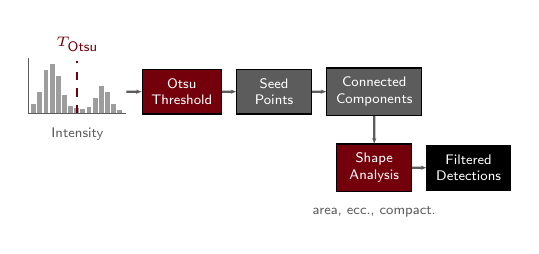
\begin{tikzpicture}[scale=0.78, every node/.style={font=\sffamily\tiny},
  block/.style={draw, fill=#1, text=white, minimum height=0.38cm,
    minimum width=0.95cm, font=\sffamily\tiny, align=center},
  block/.default={USC_Black70},
  arr/.style={-{Stealth[length=2pt]}, thick, USC_Black70}
]
  % Histogram sketch
  \begin{scope}[shift={(0,0.3)}]
    \draw[USC_Black70, thin] (0,0) -- (1.6,0); % x-axis
    \draw[USC_Black70, thin] (0,0) -- (0,0.9); % y-axis
    % Bimodal distribution bars
    \foreach \x/\h in {0.05/0.15, 0.15/0.35, 0.25/0.7, 0.35/0.8, 0.45/0.6,
                        0.55/0.3, 0.65/0.12, 0.75/0.08, 0.85/0.06,
                        0.95/0.1, 1.05/0.25, 1.15/0.45, 1.25/0.35,
                        1.35/0.15, 1.45/0.05} {
      \fill[USC_Black70, opacity=0.6] (\x,0) rectangle ++(.08,\h);
    }
    % Threshold line
    \draw[USC_Garnet, thick, dashed] (0.8,0) -- (0.8,0.85);
    \node[USC_Garnet, above, font=\sffamily\tiny] at (0.8,0.85) {$T_{\text{Otsu}}$};
    \node[below, USC_Black70] at (0.8,-0.08) {Intensity};
  \end{scope}

  % Flow blocks
  \node[block=USC_Garnet] (otsu) at (2.5,0.65) {Otsu\\Threshold};
  \node[block=USC_Black70, right=0.18cm of otsu] (seed) {Seed\\Points};
  \node[block=USC_Black70, right=0.18cm of seed] (grow) {Connected\\Components};

  % Second row
  \node[block=USC_Garnet, below=0.35cm of grow] (shape) {Shape\\Analysis};
  \node[block=black, right=0.18cm of shape] (filt) {Filtered\\Detections};

  % Shape analysis annotation
  \node[USC_Black70, font=\sffamily\tiny, below=0.06cm of shape]
    {area, ecc., compact.};

  % Arrows
  \draw[arr] (1.6,0.65) -- (otsu.west);
  \draw[arr] (otsu) -- (seed);
  \draw[arr] (seed) -- (grow);
  \draw[arr] (grow.south) -- (shape.north);
  \draw[arr] (shape) -- (filt);
\end{tikzpicture}
\end{document}
